\documentclass[11pt]{article}
\usepackage{fullpage}
\usepackage{amsmath}    % need for subequations
%\usepackage{graphicx}   % need for figures
\usepackage{verbatim}   % useful for program listings
\usepackage{color}      % use if color is used in text
\usepackage{subfigure}  % use for side-by-side figures
\usepackage{hyperref}   % use for hypertext links, including those to external documents and URLs
\usepackage[pdftex]{graphicx}
\usepackage{sidecap}
\usepackage{float}
\usepackage{wrapfig}


\title{CMSC 12300 Final Project}
\author{Andy Liu and Nelson Auner}
\begin{document}
\maketitle
\section{Introduction}

Our project investigates the use of census data to  predict whether a household self-reports that its income is over or under \$50,000. Our goals, put succintly, were to

\begin{enumerate}
  \item select  a subset of prediction methods to examine, based on interpretability of results and computational feasability
  \item test relevant models and select the best one, and,
  \item develop an accurate estimation of our model's prediction of a similar, yet different data set.
\end{enumerate}
 

To this end, we used R and Python, deployed on personal computers as well as AWS, to implement logistical regression of various combinations of regressors. We took the best models, as defined by their performance within the training set, and subjected them to cross-validation. To deal with missing data, we utilized k nearest neighbors to "fill in" missing variables with the nearest closest observation.

 Our results suggest the following: Education as a stand-alone predictor is a very good model, with around 5.4\% false positive rate and .5\% false negative rate. By very good, however, we mean compared to other non-trivial models, considering that the relative lack of diversity in our responses, given an absolute error weighting, favors a classification scheme with all-negative predictions. 


\section{Description of the Data set}
Our analysis is on the Census-Income (KDD) Data Set, a classic machine learning dataset of census data from the 1994 and 1995 Current Population Surveys conducted by the U.S. Census Bureau.

%It is also an interesting dataset for business/marketing purposes, given that predicting a household's income from semi-observeable characteristics is useful for understanding consumers for a possible product. 

The actual data is made freely available from 
\href{http://archive.ics.uci.edu/ml/datasets/Census-Income+%28KDD%29}{the UC-Irvine Machine Learning Repository}, and consists of 46 variables (see the appendix for a full list), with features such as race, capital gains, country of birth of parents, and weeks worked in the year. Because the census data is completed by participants on a voluntary basis, some variables have more missing observations than observed observations.  This is a challenging statistical problem because a household's decision to respond or not to a given question may be correlated with their household income, our choice variable of prediction. This means that normal regression methods will result in inconsistent estimators. For example, for a standard regression model $Y = X\beta$, we would have: 
\begin{equation}
E(y_i|x_i) = x_i \beta + E(y_i | x_j = NA)
\end{equation}
where $x_j$ represents the variables $j = \{j_1, j_2,...,j_k\}$ with $x_j$ not reported. Put intuitively, the second term $E(y_i | x_j = NA)$ descibes how we would alter our prediction given that we have $NA$ in columns $j$. It is possible that wealthier households are more likely to not self-report capital gains, and therefore, we should raise our expected probability of a household having annual income greater than \$50,000 if we observe a missing value.$($Another problem all-together is that households could have purposefully mis-reported-a complexity that we avoid all-together to simplify our analysis$)$. The KNN method (described later) seeks to alleviate, but does not solve this problem. Perhaps due to this interaction between household income and missing data, several variables that intuitively would be a very good measure of household income, like wage/hr, weeks worked per year, and capital gains, are not only missing in many observations, but are not good predictors of household income. 

One of the most pertinant characteristic of the data set is that the "over \$50K" variable only takes on a value of true for 6.2\% of the observations. As we noted in our original proposal, this means that a majority classifiers--predicting that income is under 50K for all observations, would have been "93.8\% accurate". However, this is not a useful predictor, since we do not know if a set of new observations would be reprentative at all of our current data. In addition, it's important to consider weighting the relative importance of assigning a false positive vs. a false negative: for a business/marketing application of the data, it may be more important to predict all of the observations with income $>$ \$50K, than correctly predict observation under \$50K. In this sense, the majority classifier is undesireable, asit predicts no observations with income $>$ \$50K, regardless of information.

\section{ Logistic Regression}
The task of predicting whether a household self reports that its income is over or under \$50,000 is a binary classification, as our outcome takes a value of either true $($income over \$50K$)$ or false $($income under \$50K $)$.  We decided early on in the project to use logistic regression, and sought to find the best classification method within the subset of logistic regression classifiers. 

\subsection{Explanation of Logistic Regression model}
Logistic regression transforms the response based on the predictors to
\begin{equation}
\pi(X) = \frac{e^{(X\beta)}}{1+e^{(X\beta)}}
\end{equation}

a transformation which looks like:
\begin{figure}[H]	
\centering
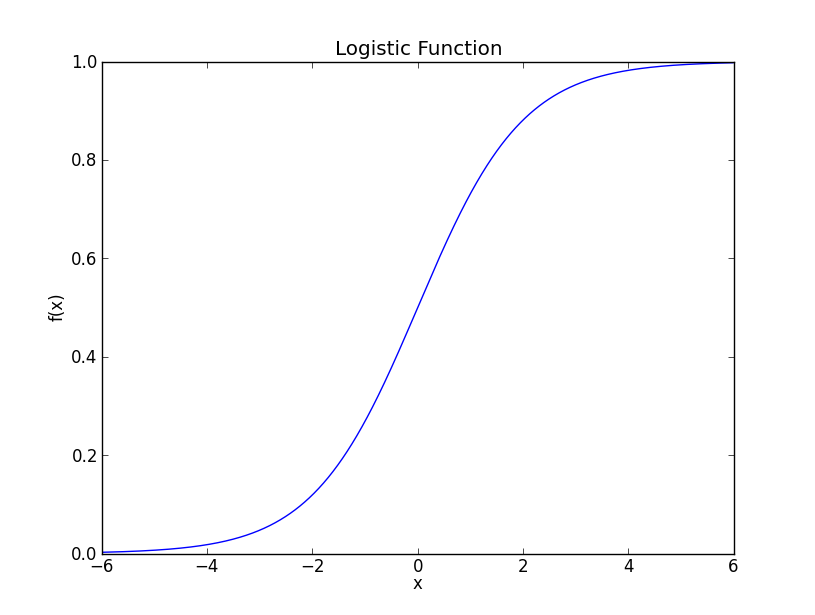
\includegraphics[width = 7cm]{logisticfunction.png}
\caption{A graph of the logistic function for reference, graphed by the authors using the numpy module of python}
\end{figure}

\subsection{Intuition behind logistic regression}
This function can be viewed as a CDF $($cumulative density function$)$ and closely mirrors that of a normal distribution, and projects the space of $X \beta$ to the interval $[0,1]$, allowing us to view the result as the probability that our outcome is 1. Our reasons for selecting a logistic regression model are simple: although it is more complicated than a basic regression mode $Y = X\beta$, logistic regression allows us to predict a binary outcome, while resulting in more interpretable coefficients $\beta$ than "black box" methods such as neural networks or random forest. 

\section{Initial analysis}
Our initial analysis was done in R, and much work was required to find and adapt the necessary statistical methods for use in python. 
We used the Akaike Information Criteria (AIC), defined as $AIC = 2k - 2ln(L)$, where $k$ is the number of the parameters in the model, and $L$ is the maximized value of the likelihood function - in our case, the logistical regression equation defined above. By maximizing AIC, we produced a subset of predictors that AIC evaluated as the "best" predictor sets. We noticed that among single-variable predictive methods, the education variable was one of the most effective, with a false positive error rate of 5\% and false negative error rate of .7\%. However, these rates are not accurate measures of performance, because we are testing our predictor with the same data we used to train. $($Correcting our evaluation of model effectiveness will be discussed in the cross validation section$)$.

\section{Filling in missing observations with 1NN}
Since we were working with somewhat cleaned census data, and all the joy that entails, one of the bigger issues that we had to deal with was missing data. Logistic regression cannot be run on an incomplete dataset. The method we decided to use to implement filling in missing data was a one nearest neighbor algorithm. The distance function we used to implement this was very simple. We selected a series of columns that were present in all observations, and the distance between any two observations was simply the number of mismatches across the various columns. The use of this distance function relies on the critical assumption that people sharing commonalities in these fields will tend to also share commonalities in the missing fields. Whether or not this is true is debateable, but the filling in missing data was useful for completeness. For every missing entry, we took its nearest neighbor, and used its column values to fill in the missing values for that entry.

In our analysis of the missing data, we realized that many of the columns that had missing data tended to involve information that does not necessarily apply to every person. For example, the field for the previous state someone lived in is not applicable to people who have lived in one state their entire lives. Due to this, we ended up dropping the majority of the columns with missing data, retaining only the columns containing information on the nationality of a person's biological parents. It would be interesting to see if our 1NN method actually led to meaningful results.

While one could argue that this method is not statistically well-founded, the fact that only two variables we use for potential logistic regressions out of many more are filled in with this method, debate over the matter seems of minimal consequence.

\section{ Results: Model Selection}
Andy also spits magic here
\section{Cross Validation}
An important aspect of our project is that our selected models predict accurately, not only for the sample for which we have data, but for the theoretical population. In this case, our population is less theoretical-it is the U.S. population represented by our census data. Because our prediction models are built by minimizing the error within our sample, it's unreasonable to assume that the model will have as low rates of error as those that are achieved by predicting the data used to generate the model.


This problem is usually addressed by the use of training sets and test sets. The data is initally partition, often around 3/4 for a training set and 1/4 for a test set. The training set is used to develop a prediction model, and the resulting model is used on the test set to obtain a theoretically unbiased estimate of model accuracy. The major downside to this approach is that valueable data points are lost when observations are assigned to the test sets, because these observations are no longer used to train the model. In situations were predictive power is important we want to minimize the loss of information that results from assigning data points to the test set. 

This is the motivation for cross validation, a procedure in which the data set is divided into k sections, or folds. For each $i = \{1,...,k\}$, a model is fit on all data excluding the $i$th fold, which is used as the test set. By repeating this procedure for all $i$, we obtain a distribution of the error without losing a information given by assigning observations to a specific test set. The below figure shows cross-validated error, divided into false positive and false negative, for a model that uses education to predict household income. The horizontal axis, labeled "k-fold" cv, is the number of folds used in CV. As the number of folds increases, the size of the training set in each iteration increases, and, in general, model accuracy improves. The vertical axis displays the percentage of error. 
\begin{figure}[H]
\centering
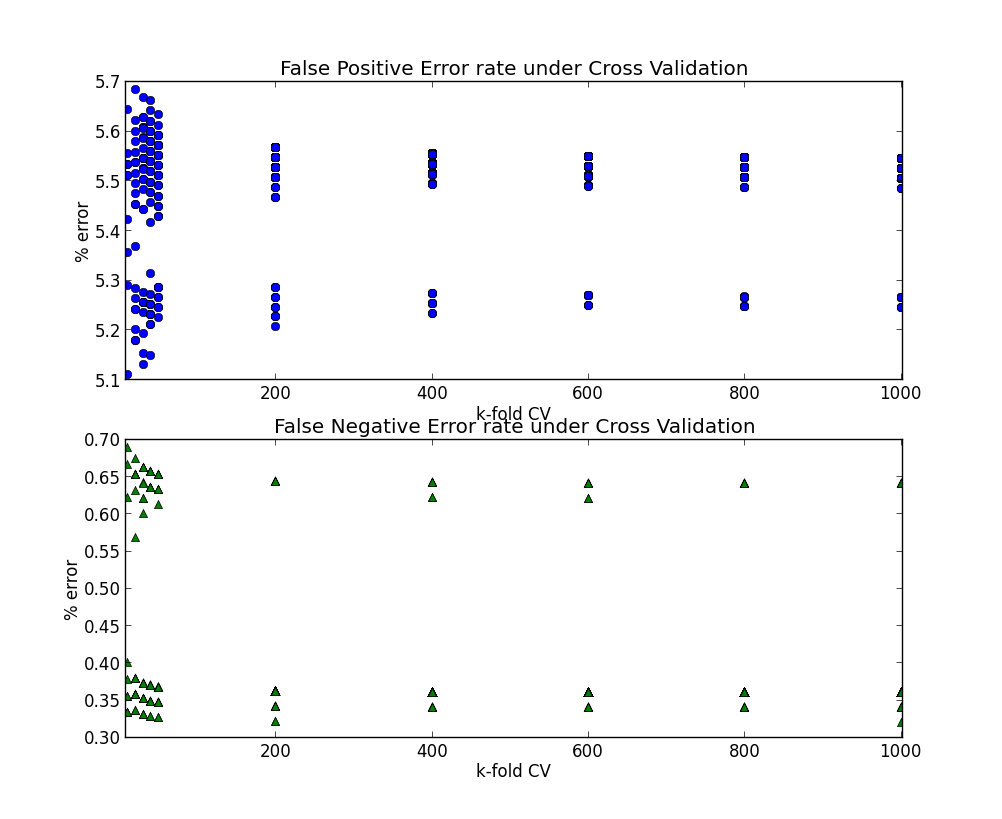
\includegraphics[width = 12cm]{CV_5K_1Kfold.png}
\caption{Error rate of education-only model, performed on 5,000 randomly selected observations}
\end{figure}

A couple of things to note from the results: Although increasing the number of folds seems to decrease the error rate for small k, we do not observe a visible decrease in the error rate for larger k. In addition, we notice a large spread across iterations for the same k-fold CV procedure. This is likely due to the limited variance in our outcome variable-within this 5,000 sample of our data, the number of households with self-reported income over \$50,000 was less than 100. If a couple of difficult-to-predict observations-say, with low education but high income-are placed (by chance) into one specific fold, the error for that fold will be significantly higher than other folds. This is our hypothesis, cannot be examined further given our dataset, and merits further investigation.

Another issue that we wanted to investigate with cross validation was the effect of filling in missing observations using KNN. 
One member of our team was doubtful that this method would improve the accuracy of our model. To the contrary, filling in observations using data from other observation, that are included in the training set, doesn't seem to add any new information, and might decrease the quality of the model with added variance by making claims on observation with filled-in data. 

The below figure shows a similar cross validation procedure, applied to a 5,000-observation sample of the data after having applied the KNN-fill-in-missing-data procedure:
\begin{figure}[H]
\centering
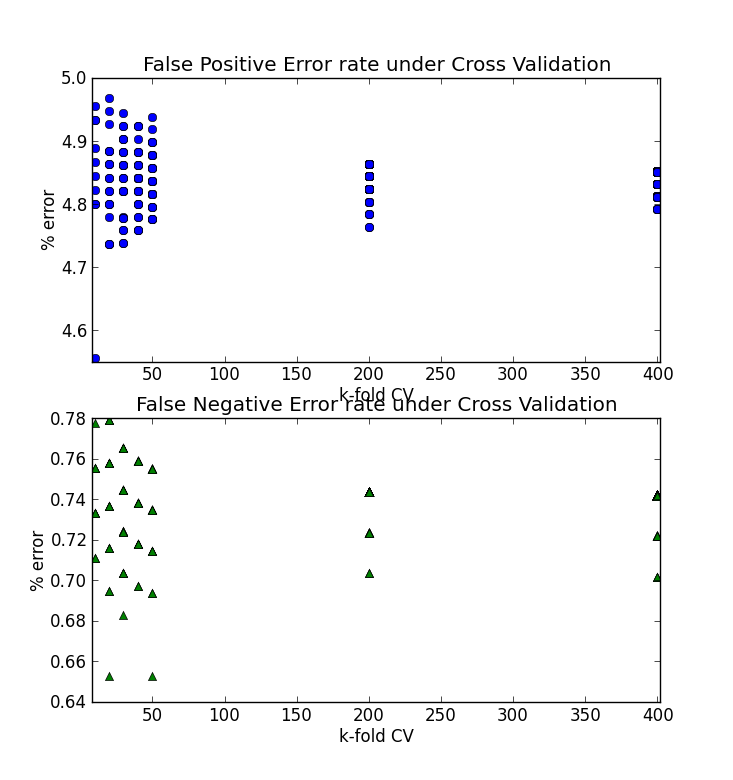
\includegraphics[width = 12cm]{CV_5K_400fold_filled.png}
\caption{Error rate of education-only model, performed on 5,000 randomly selected observations after filling in missing variables with KNN}
\end{figure}

The results are extremely interesting for a couple of reasons. We note that compared to the non-filled-in data, the false positive rate is much lower $($ an average of 4.8\%compared to 5.4\%$)$ and the false negative rate is slightly higher $($ .72\%compared to .5\%$)$.  Besides the level of error, the relationship between number of folds and error rates also seems to be different for filled-in data vs. the original data. Looking at the original data, the error rates do not visibly converge. even at 1000-fold CV, there is a .3\% range in false positive and false negative error rate between folds. Looking at the cross validation on filled-in data, we see that error rates are more closely clustered, despite the fact that CV was only performed up to 400 folds for the filled-in data, and up to 1000 folds for the original data. 

Finally, how might our results of cross-validation change with respect to the size of the data. The previous simulations mentioned were performed on a randomly-selected, 5,000-observation subset of the data. To investigate, we performed the same CV procedure on the entire dataset. This was incredibly computationally-expensive, as the computational complexity of cross validation performed over a number of folds increases exponentially with respect to the number of observations in the data. To ameliorate the computational cost of the simulation, computation was distributed $($manually$)$ among multiple machines, and indinvidual results were combined.  The below figure shows the result of the simulation:
\begin{figure}[H]
\centering
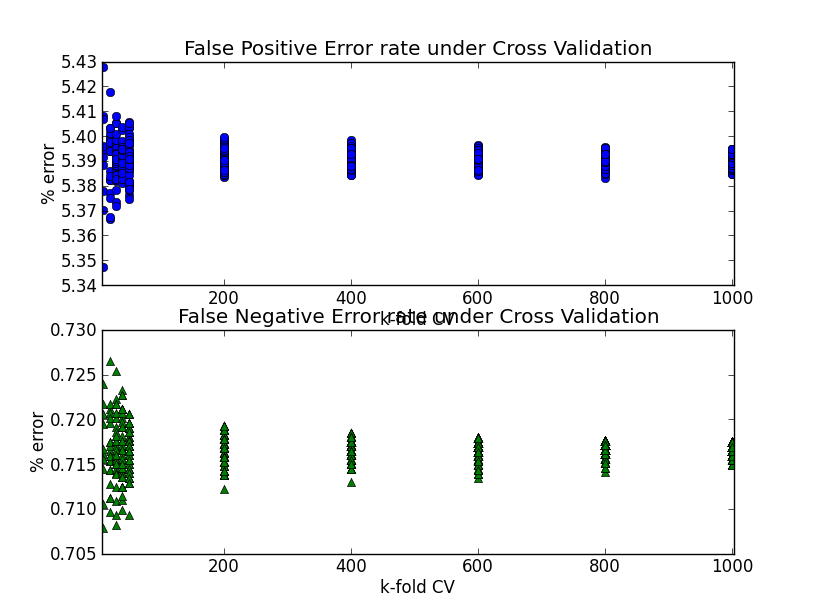
\includegraphics[width = 12cm]{CV_FULLn_1Kfold.png}
\caption{Error rate of education-only model, performed on the entire dataset over various fold sizes}
\end{figure}

Compared to Figure 2, the results of the simulation


\section{appendix}
For a list of the variables in the data set, see 

\end{document}